%
% this file is encoded in utf-8
% v1.7

%%% 參考文獻
\newpage
%\bibliographystyle{unsrt}
\cleardoublepage
\phantomsection
\addcontentsline{toc}{chapter}{\nameRef}
\renewcommand{\bibname}{\protect\makebox[5cm][s]{\nameRef}}
%  \makebox{} is fragile; need protect
%\bibliographystyle{unsrt} 
\bibliographystyle{ieeetr}  % 使用 IEEE Trans 期刊格式
%\bibliographystyle{unsrt}
\bibliography{my_bib}  %reference 所需的bib檔
%\bibliographystyle{unsrt} 

%%% 附錄
%
% this file is encoded in utf-8
% v1.7
%%% 每一個附錄 (附錄一、附錄二、...) 都要複製此段附錄編排碼做為起頭
%%% 附錄編排碼 begin >>>

\includepdfset{pages=-,pagecommand=\thispagestyle{AppendixPage}}

\newpage
\chapter*{附錄一:典型校舍初步評估表} % 修改附錄編號與你的附錄名
\label{appendix-pe}
\addcontentsline{toc}{chapter}{附錄一:典型校舍初步評估表} %建議此內容應與上行相同
\renewcommand{\thechapter}{一} % 如果是附錄二,則內容應為{二}

\setcounter{equation}{0} 
\setcounter{figure}{0} 
\setcounter{footnote}{0} 
\setcounter{section}{0} 
\setcounter{subsection}{0}
\setcounter{subsubsection}{0}
\setcounter{table}{0} 
%%% <<< 附錄編排碼 end

% 附錄內容開始
見下頁。

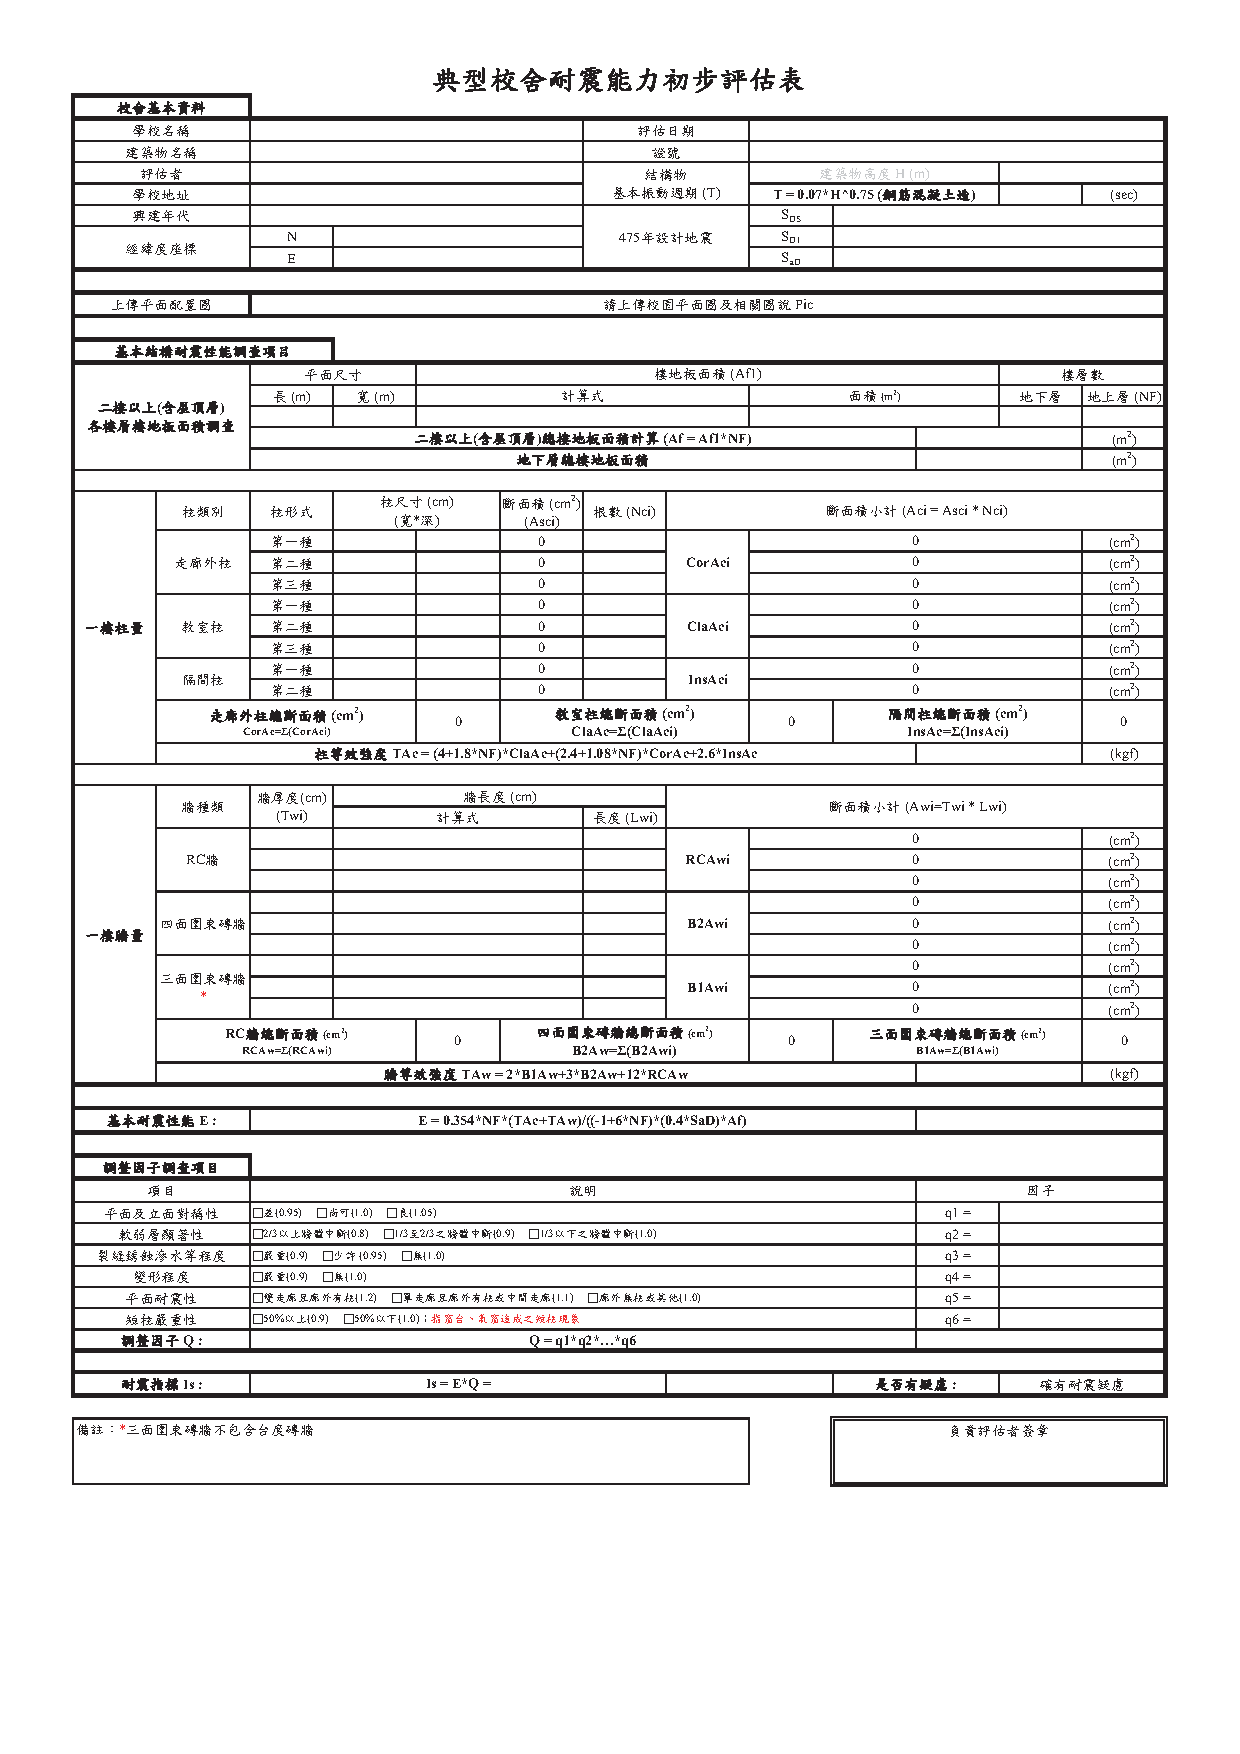
\includepdf[fitpaper=true,scale=0.95]{appendix/20120516-Preliminary-Typical.pdf}

%%% 如果有附錄二、三、...,則在此繼續加上「附錄編排」碼
% 每一個附錄會自動以新頁開始

\newpage
\chapter*{附錄二:典型校舍詳細評估表} % 修改附錄編號與你的附錄名
\label{appendix-de}
\addcontentsline{toc}{chapter}{附錄二:典型校舍詳細評估表} %建議此內容應與上行相同
\renewcommand{\thechapter}{二} % 如果是附錄二,則內容應為{二}

\setcounter{equation}{0} 
\setcounter{figure}{0} 
\setcounter{footnote}{0} 
\setcounter{section}{0} 
\setcounter{subsection}{0}
\setcounter{subsubsection}{0}
\setcounter{table}{0} 
%%% <<< 附錄編排碼 end

% 附錄內容開始
見下頁。

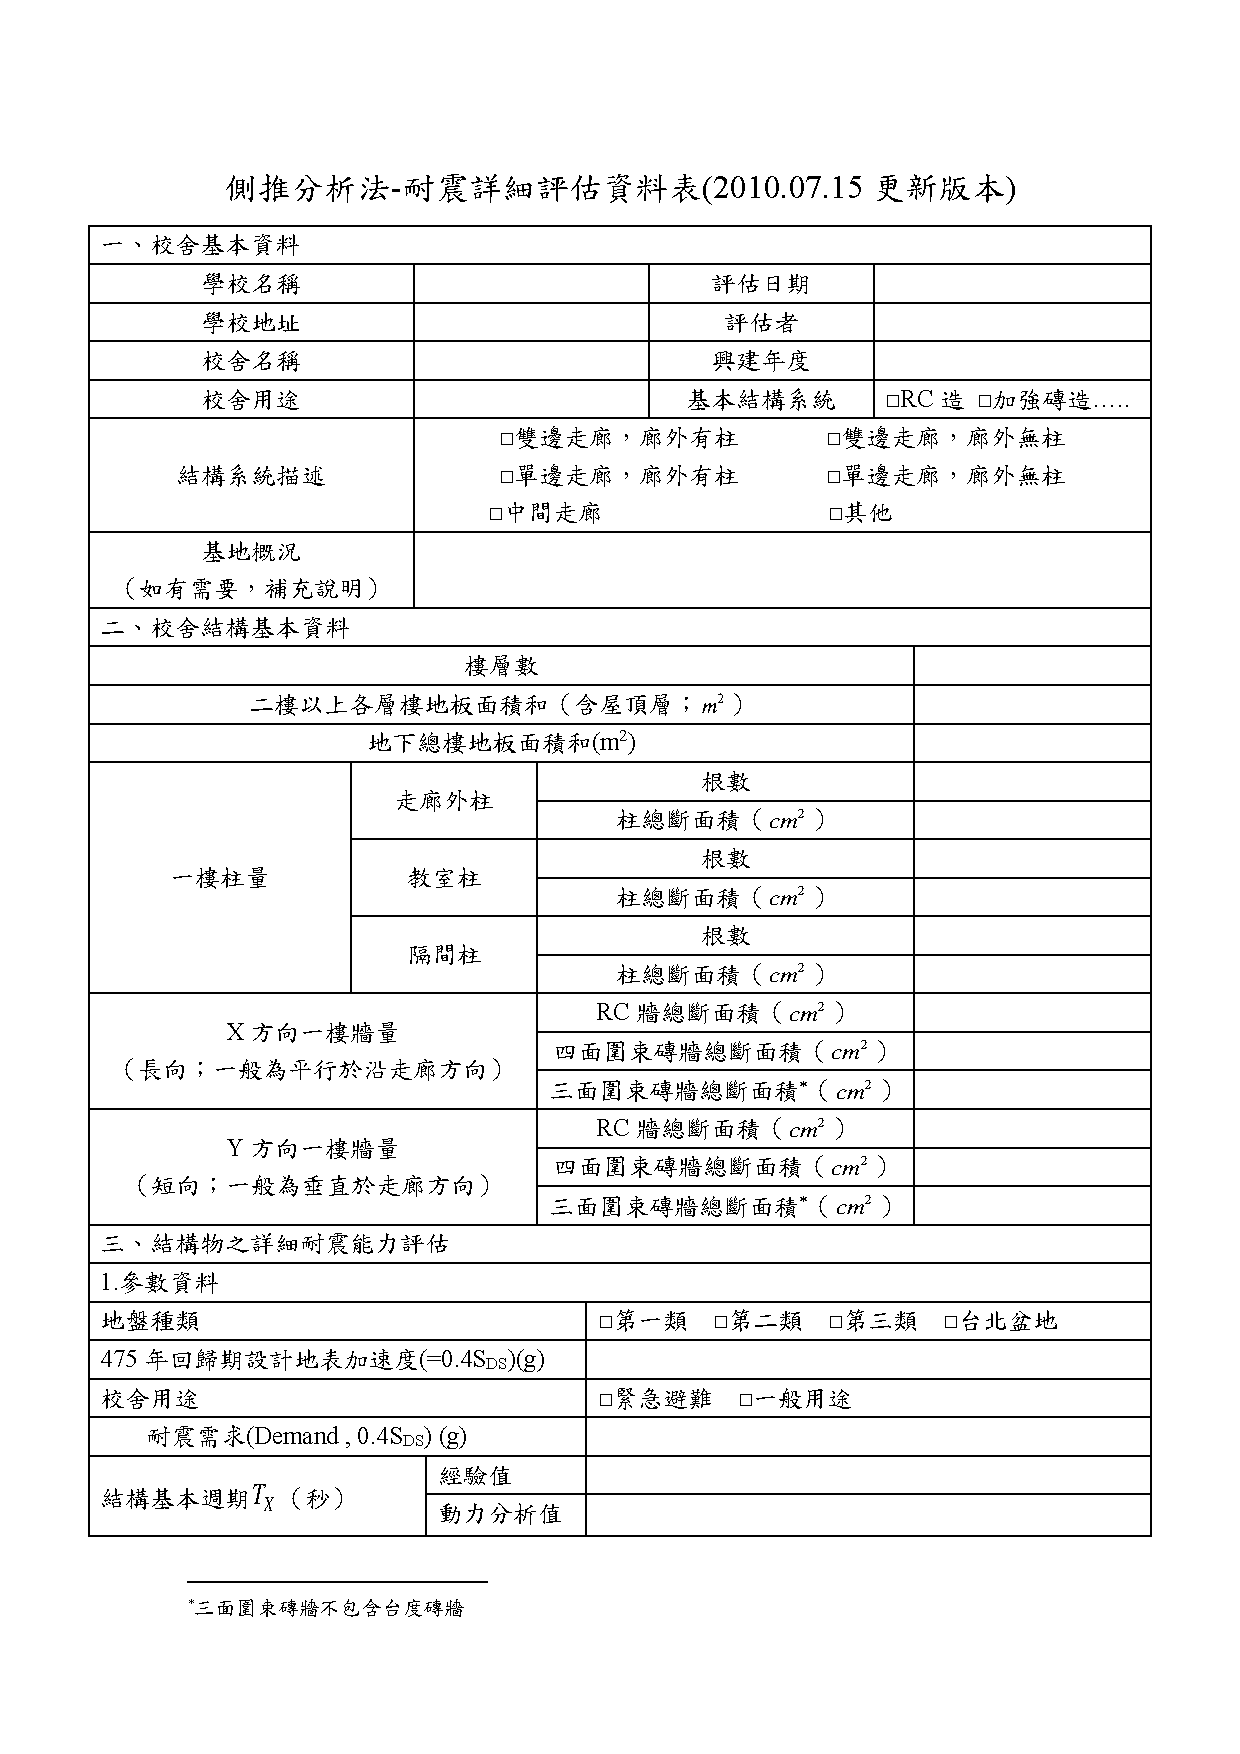
\includepdf[fitpaper=true,scale=0.95]{appendix/detailed-evaluation.pdf}


\newpage
\chapter*{附錄三:典型校舍補強設計表} % 修改附錄編號與你的附錄名
\label{appendix-re}
\addcontentsline{toc}{chapter}{附錄三:典型校舍補強設計表} %建議此內容應與上行相同
\renewcommand{\thechapter}{三} % 如果是附錄二,則內容應為{二}

\setcounter{equation}{0} 
\setcounter{figure}{0} 
\setcounter{footnote}{0} 
\setcounter{section}{0} 
\setcounter{subsection}{0}
\setcounter{subsubsection}{0}
\setcounter{table}{0} 
%%% <<< 附錄編排碼 end

% 附錄內容開始
見下頁。

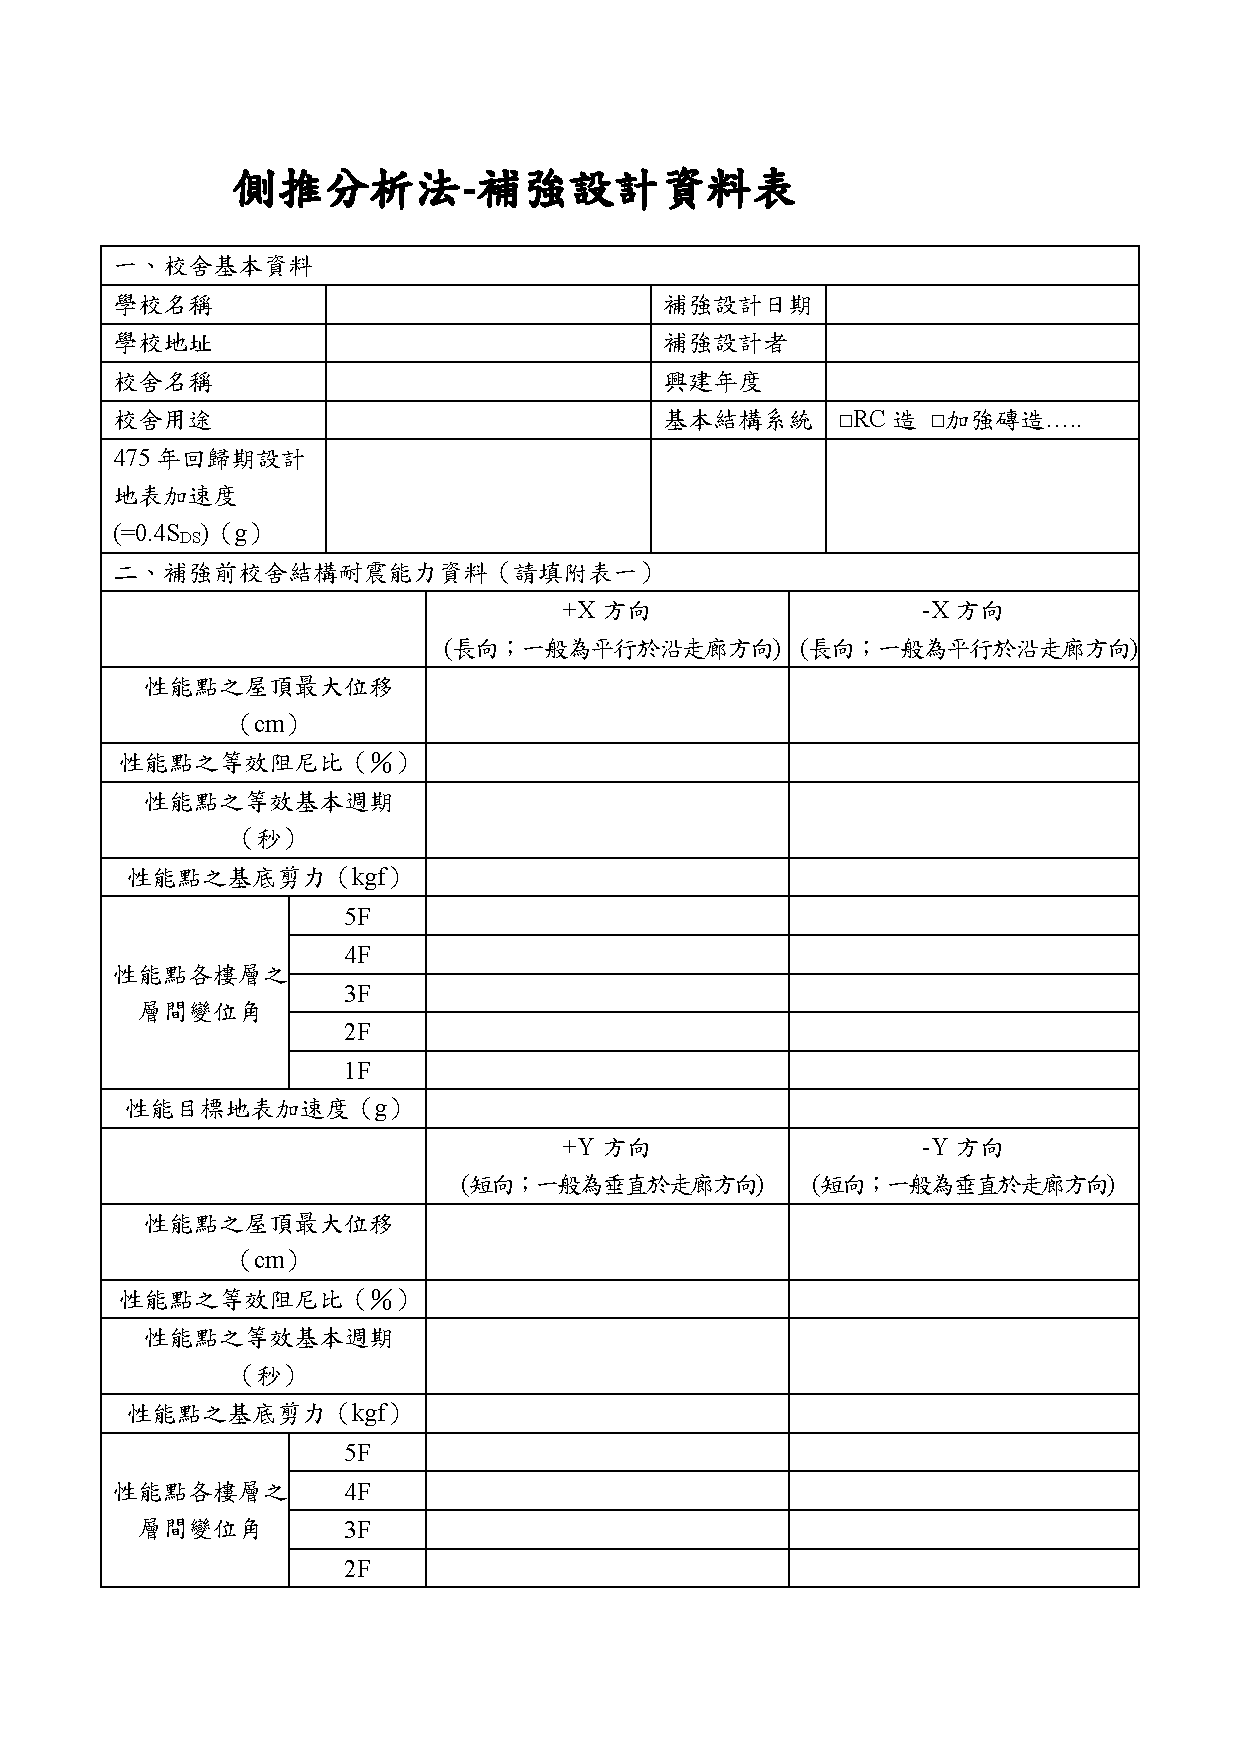
\includepdf[fitpaper=true,scale=0.95]{appendix/retrofit.pdf}

%%% 自傳
%\newpage
%\chapter*{\protect\makebox[5cm][s]{\nameVita}} % \makebox{} is fragile; need protect
%\addcontentsline{toc}{chapter}{\nameVita}
%本人生於 1981 年 1 月 1 日,在桃園內壢。家裡經營電器行,上有一位姊姊。從小就喜歡拆解店裡收回的報廢家電用品,練就了一身好手藝與探究一切的好奇心。

國小就讀平鎮國小。由於把供應全校用水的抽水馬達拆開研究裝不回去,造成全校停水,廁所污穢不堪。被校長處罰掃廁所一個星期。那真是我少時年幼無知的一頁插曲。



%%%%%%%%%%%%%%%%%%%%%%%%%%%%%%%
%       授權書 (計頁碼,但不印頁碼) 
%%%%%%%%%%%%%%%%%%%%%%%%%%%%%%%
%
% insert the printed standard form when the thesis is ready to bind
% 在口試完成後,再將已簽名的授權書放入以便裝訂
% create an entry in table of contents for 授權書
% 目前送出空白頁
\cleardoublepage
\phantomsection
%
\includepdf[fitpaper=true,scale=1,pagecommand=\thispagestyle{empty}]{backpages/G-15.pdf}

\includepdf[fitpaper=true,scale=1,angle=90,pagecommand=\thispagestyle{empty}]{backpages/img-122151637-0001.pdf}

